
\subsection{Overview and UML Diagram}

The processor is the simulation engine inside YAMS. 

The processor reads machine code instructions from the memory, decodes and executes them. It models a MIPS R3000 CPU, which has a RISC architecture and all instructions are 32 bits in length. This length is called a MIPS machine word. The following diagram shows the software components that go to make up the processor.

\begin{figure}
\begin{center}
\includegraphics[width=8cm]{processor-overview.eps}
\caption{The Components of the YAMS Processor}
\end{center}
\end{figure}

This UML diagram shows how the components are implemented as interfaces and classes. The package that all processor classes may be found in is called 'yams.processor'.

\begin{figure}[p]
\begin{center}
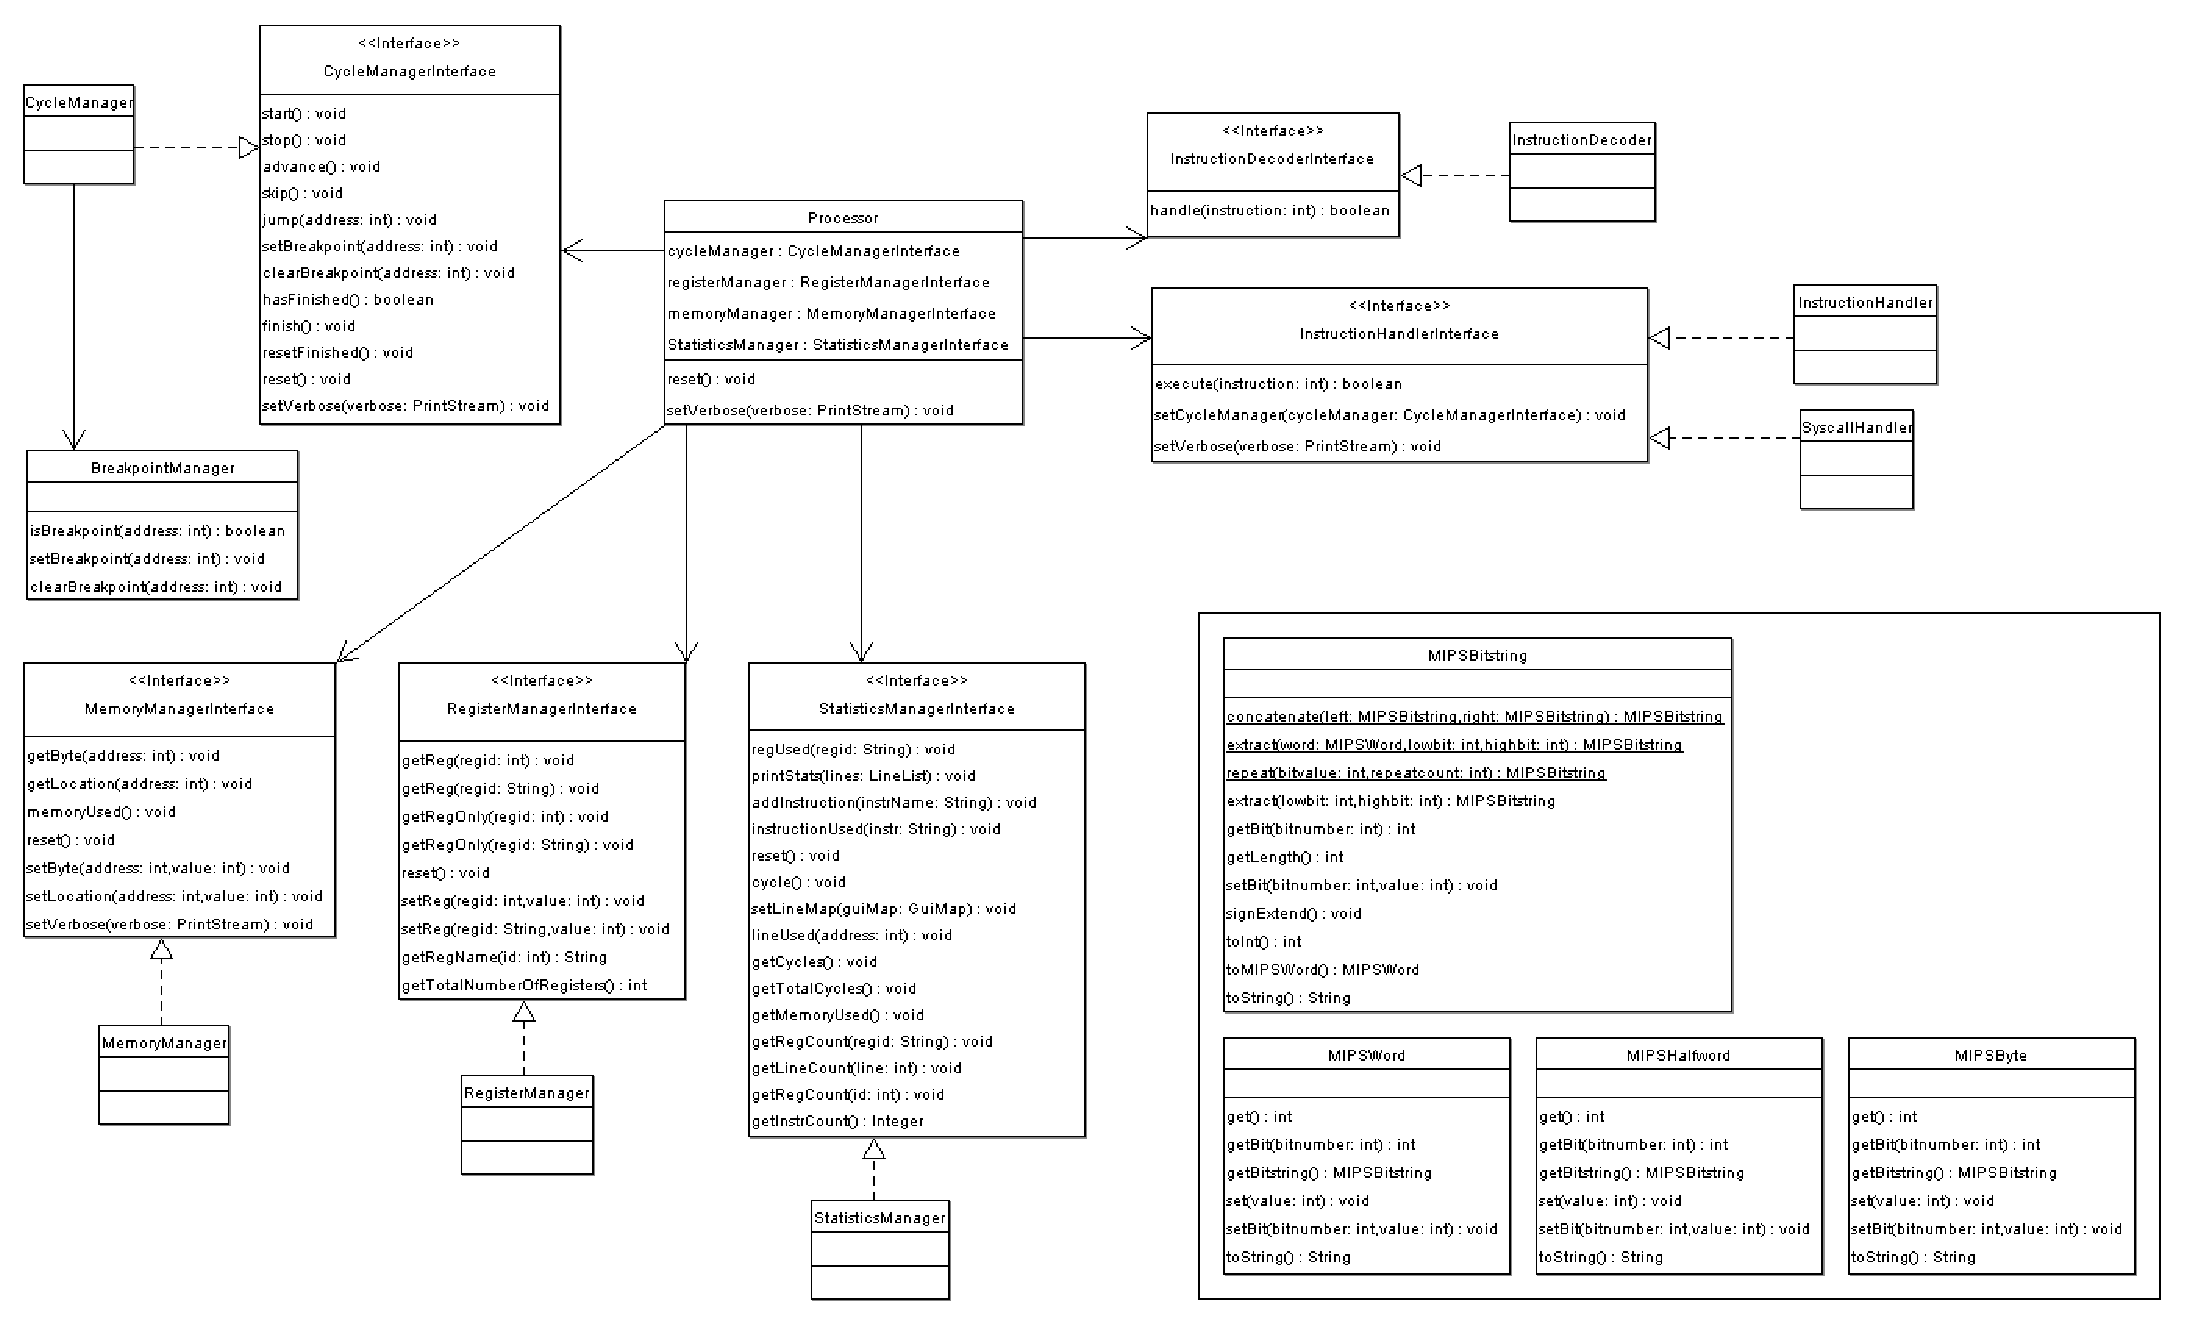
\includegraphics[angle=90,width=10cm]{processor-uml.eps}
\caption{The UML Diagram of the Procesor Classes and Interfaces}
\end{center}
\end{figure}


The processor is capable of recognising and executing any instruction present in the XML repository. Example instructions are: mul (performs multiplication), add (performs addition), beq (performs branch if equal) and syscall (performs system call). After an instruction is executed, the state of the processor will be exactly as described by the instruction file. For example, after an 'add' instruction, the value in the destination register will be the result of the addition of the two other operands.

The processor exposes interfaces for each Manager component above, so it is simple to get information about any aspect of the state held by the processor. The processor also keeps many statistics on what has been executed.


\subsection{Using the Processor}

The entrypoint to the processor is the 'Processor' class. Create a new Processor object using the following constructor:

public Processor(YAMSController yamscontroller, InputStream in, PrintStream out, PrintStream verbose)

This will instantiate and initialise each class that is a processor component in turn. Each class with a responsibility to print or receive input has the appropriate Input or PrintStream(s) passed to it. 
The passed InputStream 'in' will be used for any textual input required from the user, the PrintStream 'out' is used for program output and the PrintStream verbose is used for extended execution information, such as the names of instructions.

The processor exposes four managers as public attributes: cycleManager, registerManager, memoryManager, and statisticsManager.
To begin execution, the processor object's cycle manager should be told to jump(addr) to the start of code. Then the cycle manager's advance() method should be called to execute individual instructions, or start() to execute until completion. Completion occurs when an exit 'syscall' instruction is executed.
The YAMS console and GUI perform this transparently to the user.


\subsection{The Manager Classes}

Each Manager class (with the exception of the BreakpointManager) implements a similarly-named interface.

\subsubsection{CycleManager}

The cycle manager sequences the operation of each instruction cycle, and the following diagram shows most of one such cycle.


\begin{figure}
\begin{center}
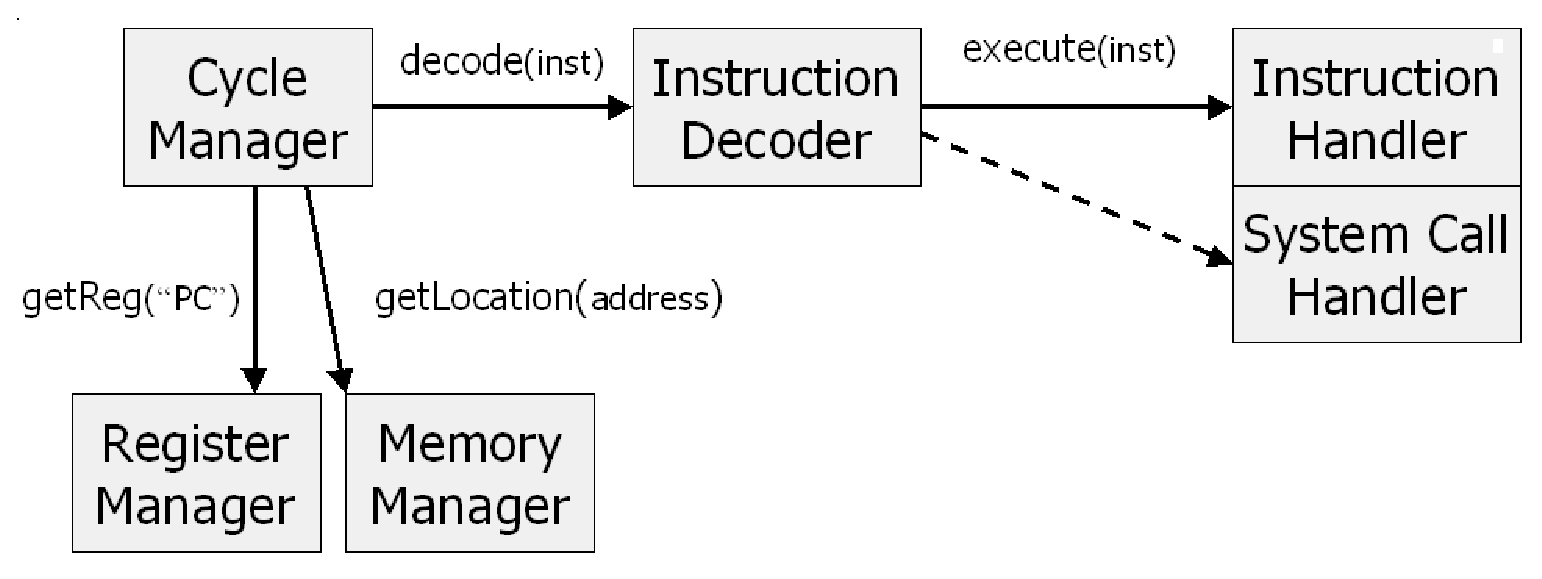
\includegraphics[width=8cm]{processor-cycle.eps}
\caption{Execution of a Single Instruction}
\end{center}
\end{figure}


First, the cycle manager gets the current value of the program counter. The memory manager is then asked for the machine word at the memory location corresponding to that value. The word, an instruction, is passed to the instruction decoder which determines which handler should execute it. The instruction is executed by the appropriate handler and the state of the MIPS registers and memory is affected as a result. Finally, and not shown, the program counter is incremented to point to the next instruction instruction in memory, and the statistics manager is updated.

The methods to control execution are:
jump(int address) - sets the program counter to the given address
start() - runs until a 'syscall' exit is encountered
stop() - stops the processor after the current cycle finishes execution
advance() - when stopped, execute the next instruction 
skip() - when stopped, skip over the next instruction

The cycle manager also supports breakpoints. When a breakpoint is encountered, the cycle manager stops execution before the instruction at the address of the breakpoint is executed. The BreakpointManager class maintains the list of breakpoints for the cycle manager. The breakpoints are held in a HashSet.

The cycle manager maintains a series of flags, to tell the controller (console or GUI) whether it is currently running (executing instructions) and if an exit 'syscall' has been executed. The reset() method can be invoked to reset these flags.

\subsubsection{RegisterManager}

The register manager simulates the registers that are available to the MIPS processor.  There are 32 generic registers available to use, and 3 special registers \verb"$PC", \verb"$LO" and \verb"$HI".

The register manager uses treemap data structures as they have fast access times.  When it is created before the run of the program, the registers are loaded into the treemap with a 0 count.

There are then access procedures to get and set values for the registers.  The value currently in a register is returned if a get request is made, or set with a specified value if a set request is made.  Each time a register is accessed, a method in the statistics manager is called to update the usage count for that
register.  There are also access procedures that do not call the statistics manager, this is for when the content of a register needs to be read by the simulator, for example while displaying values in the GUI.

There is also a reset procedure to reset all of the values to 0 making the register manager ready for the next run program.

\subsubsection{MemoryManager}

The Memory Manager simulates the memory available to the MIPS processor.  It is assumed that initially all the memory locations are set to 0.  The memory is split up into 3 segments - reserved, text and data.

When the memory manager is created, the divisions of these sectors can be specified in the constructor, if these are invalid, the default segmentation is used.

The memory manager uses tree map data structures, one for each memory segment, as these have fast access times.  The objects held in the treemaps are of type MIPSWord which can store 32bits and have various manipulation procedures making it easy to change the values and bits held in each.  There are access procedures to get and set memory words, and also the same procedures to get and set individual bytes in memory.

When an incoming request is made to get or set a location, the address given is used to resolve the treemap that it corresponds to.  The location value is then returned if it is a get request, or set with the supplied value if it is a set request.

There is also a reset procedure which clears the treemaps ready for the next program to be run.  Since it is assumed that all value in memory are initially zero, it is not necessary to store all locations in the treemap - any request that is made for a location not stored in the map will just return 0.

\subsubsection{StatisticsManager}

The statistics manager keeps a record of various statistics that are updated as the program is executed.  These are:

\begin{description}
\item[Line execution count] Showing how many times each line of the assembly file has been executed.
\item[Instruction count] Giving how many times each instruction has been used in the program.
\item[Register usage count] Showing how many times each register has been used in the program
\item[CPU Cycles] required to run the program
\item[Total memory] in words taken up by the program
\end{description}

The class uses tree maps to store the counts as these are ordered and fast to access.  The CPU Cycles and Total Memory are just stored in variables.

\begin{description}
\item[Line Execution Count]
For the line execution count, the statistics manager needs a reference to the GUIMap class in the assembler which maps memory addresses to line numbers.  Every time the Cycle Manager cycles, it passes the statistics manager the value of the program counter.  The GUIMap is then used to resolve this address to a line number, so the line execution count can then be incremented.

\item[Instruction Count]
When the instructions are initially loaded by the assembler from the XML instruction file, the names are also loaded into the statistics manager so the counts can be tracked for each program run.  

When the instruction handler executes an instruction, a method is called in the statistics manager with the name of the instruction.  This then updates the usage count for that run of the program.

\item[Register Usage Count]
The register usage count is incremented by an access procedure called by the register manager each time a register is accessed.

\item[CPU Cycle Count]
The CPU cycle count is incremented by an access procedure called by the cycle manager on every cycle.

\item[Total Memory]
The total memory in words is given by calling an access procedure in the memory manager that returns the total size of all 3 memory maps held.

\item[Reset]
There is also a reset procedure to set all the statistics to 0 ready for the next program to run.  For performance, the instructions names are not deleted from the instruction count treemap so they do not have to be loaded from the XML each time a new program is run. Instead the counts are just set to 0.
\end{description}



\subsection{The Instruction Execution Classes}

\subsubsection{InstructionDecoder}

The instruction decoder in the processor determines which handler should execute a given instruction. 'Syscall' instructions are executed in the syscall handler, and all other types execute in the instruction handler.

Both handlers implement the InstructionHandlerInterface, which contains the execute(int instruction) method that the instruction decoder invokes.

\subsection{InstructionHandler}

This class is one of the most important in all of YAMS, since it forms the point of execution of 
99\% of instructions.

In order to understand how instructions can be decoded and executed, the format of MIPS instructions must be understood. MIPS instructions can be broadly classed into 3 types:

\begin{description}
\item[R types] which only operate on registers e.g. add rd, rs, rt
\item[I types] which have an immediate operand e.g. lui rd, imm
\item[J types] which are jump instructions with an address e.g. j label1
\end{description}

The characteristics of the instruction types, so that they can be detected and decoded, are shown in table \ref{tab:InstructionCharacteristics}

\begin{table}
\begin{center}
	\begin{tabular}{|l|l|}
	\hline
	R type	&	The 'op' field (bits 26..31) are 000000 \\
			&	The 'func' field (bits 0..5) uniquely identifies the instruction \\
	I types	&	The 'op' field (bits 26..31) uniquely identifies the instruction \\
	J types	&	As for I types, the 'op' field (bits 26..31) uniquely identifies the instruction \\
	\hline
	\end{tabular}
\caption{Instruction Characteristics}
\label{tab:InstructionCharacteristics}
\end{center}
\end{table}

When the \verb"execute()" call is invoked, an instruction to be executed is passed to the instruction handler. The handler tests it to see whether it has 000000 for its 'op' field, and thus whether it is an R type instruction. Otherwise it is an I or J type instruction.
Once the broad type of the instruction is determine, the operands are decoded from the instruction.
Not all operands are used in every instruction.

MIPS instruction operands are shown in table \ref{tab:InstrOps}.

\begin{table}
\begin{center}
	\begin{tabular}{|l|l|}
	\hline
	R types	&	rd (5 bit register identifier) \\
			&	rs (5 bit register identifier) \\
			&	rt (5 bit register identifier) \\
			&	shamt (5 bit shift amount) \\
			&	func (instruction identifier) \\
	I types	&	rs (5 bit register identifier) \\
			&	rt (5 bit register identifier) \\
			&	imm (16 bit immediate) \\
	J types	&	addr (26 bit register identifier) \\
	\hline
	\end{tabular}
\caption{MIPS Instruction Operands}
\label{tab:InstrOps}
\end{center}
\end{table}
		
Then for an R type, the value of the 'func' field is compared against all the R type instructions in the instruction handler, and the correct MIPS instruction is executed using the operands as extracted above.
For an I or J type, the 'op' field is compared against the all the I \& J type instructions in the instruction handler, and the correct MIPS instruction is executed using the operands as extracted above.

If the instruction to be executed cannot be handled by the instruction handler, then an YAMSUnsupportedInstructionException is thrown. This would be the case, for example, if a floating point instruction was executed by an instruction handler with no floating point instruction support.

\subsubsection{instructionHandler.xslt}

Not a single instruction is hard-coded in YAMS. It would be undesirable and inflexible to do so. Instead, the XML repository's instruction file is used to produce an instruction handler at compile time through an XSLT transformation.
When YAMS is built, \verb"yams.auto.xslt.instructionHandler.xlst" is applied to the XML repository, \verb'Instruction_file.xml', and the transformation produces as output a Java source file: \verb'yams.processor.InstructionHandler.java'
This output Java file is compiled in with all other YAMS sources during the build process.

The instruction handler's XSLT transformation contains the template for an instruction handler class, but without any instructions present. Java code is produced for each separate instruction as if-statements, which are then added to the template instruction handler to form the generated instruction handler. 

The transformation determines for each instruction detailed in the XML file, whether it is an R or I/J type. If it is an R type, it extracts the 'func' bitfield from the instruction's machine code representation and creates an if-statement to detect an R type instruction with that 'func' value. 
If it is an I/J type it extracts the 'op' bitfield instead and creates an if-statement to detect an I/J type instruction with that 'op' value.

Inside the if-statement, a statement is added to print the instruction name to the verbose PrintStream, and another to inform the statistics manager that an instruction of that name is being executed. 

The Javacode associated with the instruction is placed inside the if-statement, so that the semantics of the instruction are exactly executed. Finally, a 'return true' is added and the if-statement is closed.

An example follows. 

SOURCE:  Pertinent tags for 'add' instruction in XML file, \verb"Instruction_file.xml"

\begin{verbatim}
<Instruction>
  <Name>add</Name>
  ...
  <Javacode>
  regs.setReg(rd, regs.getReg(rs) + regs.getReg(rt));
  </Javacode>
  <Type>Extended</Type>
  <CoreMachineCode>000000bbbbbcccccaaaaa00000100000</CoreMachineCode>
  ...
</Instruction>
\end{verbatim}

OUTPUT:  If-statement for 'add' instruction in generated \verb"InstructionHandler.java"

\begin{verbatim}
if(func == toDecimal("100000")) {
  verbose.println("add");
  stats.instructionUsed("add");

  regs.setReg(rd, regs.getReg(rs) + regs.getReg(rt));

  return true;
}
\end{verbatim}


\subsubsection{SyscallHandler}

The Syscall Handler only handles the 'syscall' instruction. This instruction is special because it can communicate with the operating system, that is, the 'outside world' to the simulator. Examples of uses are to print a string to the console, or read a number from the user.

The value in register \$v0 is the system call code, the 'syscall' instruction performs a different function depending on this code.

\begin{table}
\begin{center}
	\begin{tabular}{|l|l|l|l|}
	\hline
	Service			&	Code	&	Arguments				&	Result \\
	\hline
	print\_int		&	1		&	\$a0 = integer			& \\
	print\_float	&	2		&	\$f12 = float			& \\
	print\_double	&	3		&	\$f12 = double			& \\
	print\_string	&	4		&	\$a0 = string			& \\
	read\_int		&	5		&							&	integer (in \$v0) \\
	read\_float		&	6		&							&	float (in \$f0) \\
	read\_double	&	7		&							&	double (in \$f0) \\
	read\_string	&	8		&	\$a0 = buffer, \$a1 = length	& \\
	sbrk			&	9		&	\$a0 = amount			&	address (in \$v0)  \\
	exit			&	10		&							&	\\
	\hline
	\end{tabular}
\caption{System Calls}
\label{tab:SystemCalls}
\end{center}
\end{table}


\subsubsection{SYSCALLHANDLER.XSLT}

Like for the instruction handler, the XML repository's instruction file is used to produce a syscall handler at compile time through an XSLT transformation.
When YAMS is built, \verb'yams.auto.xslt.syscallHandler.xlst' is applied to the XML repository, \verb'Instruction_file.xml', and the transformation produces as output a Java source file: \verb'yams.processor.SyscallHandler.java'
This output Java file is compiled in with all other YAMS sources during the build process.

The syscall handler's XSLT transformation contains the template for an syscall handler class, but without any instructions present. Java code is produced for the syscall instruction as an if-statement, which is added to the template syscall handler to form the generated syscall handler. 

The syscall handler's transformation only produces code for the 'syscall' instruction, all other instructions are ignored, since they are catered for by the instruction handler.

It may be argued that the separation of the instruction and syscall handlers is only a logical separation, but the YAMS developers believed it was a good idea to have the potentially exotic syscalls to be in a source file of their own.

\subsection{The Bitstring Classes}

\subsubsection{MIPSBitstring}

The processor helper classes were developed to help with bitstring and binary operations.
The MIPSBitstring class represents bitstrings, that is, sequences of binary digits. It supports concatenation and splitting of bitstrings, as well as giving decimal integer representations. This class is used extensively to extract and test bitfields inside MIPS instructions. It can also provide sign-extended decimal integer representations of bitstrings, which is very useful for converting a 16-bit two's complement immediate into a 32-bit signed Java int.

\subsubsection{MIPSByte, MIPSHalfword, MIPSWord}

The Java int datatype is used throughout YAMS as a 32-bit integer, that can represent a MIPS machine word. The MIPSWord class (and similarly for its smaller-width sister classes) is a wrapper for the MIPSBitstring so that the machine word has simple get() and set() methods, as well as bit manipulation and bitstring extraction methods.
